\documentclass[11pt,a4paper]{article}
\usepackage[margin=2.15cm]{geometry}
\usepackage[T1]{fontenc}
\usepackage[utf8]{inputenc}
\usepackage{array,booktabs,tabularx,hyperref,listings,xcolor,titlesec,parskip,tikz}
\usepackage[expansion=false]{microtype}
\usetikzlibrary{arrows.meta,positioning,shapes.geometric}

% ---- palette ---------------------------------------------------------------
\definecolor{leafcyan}{RGB}{0,140,140}
\definecolor{leafgreen}{RGB}{60,150,95}
\definecolor{leafamber}{RGB}{214,142,45}
\definecolor{leafred}{RGB}{185,72,72}
\definecolor{leafink}{RGB}{36,42,48}
\definecolor{leafmuted}{RGB}{92,104,114}
\definecolor{leafpanel}{RGB}{245,248,248}
\definecolor{leafline}{RGB}{205,218,218}
\definecolor{leafcode}{RGB}{241,244,244}

\hypersetup{colorlinks=true,linkcolor=leafcyan,urlcolor=leafcyan,citecolor=leafcyan}

% ---- listings --------------------------------------------------------------
\lstdefinestyle{leaf}{
  basicstyle=\ttfamily\footnotesize,
  breaklines=true,
  backgroundcolor=\color{leafcode},
  frame=single,
  rulecolor=\color{leafline},
  xleftmargin=8pt,
  xrightmargin=8pt,
  aboveskip=7pt,
  belowskip=7pt,
  showstringspaces=false,
}
\lstset{style=leaf}

% ---- section formatting ----------------------------------------------------
\titleformat{\section}{\Large\bfseries\color{leafcyan}}{}{0pt}{}[\titlerule]
\titleformat{\subsection}{\large\bfseries\color{leafink}}{}{0pt}{}
\titleformat{\subsubsection}{\normalsize\bfseries\color{leafmuted}}{}{0pt}{}

% ---- visual helpers --------------------------------------------------------
\newcommand{\metricbox}[3]{%
  \fcolorbox{leafline}{leafpanel}{%
    \begin{minipage}[t][2.1cm][c]{0.29\linewidth}
      \centering
      {\Large\bfseries\color{leafcyan} #1}\\[-1pt]
      {\bfseries #2}\\[-1pt]
      {\footnotesize\color{leafmuted} #3}
    \end{minipage}}}

\newcommand{\statusbox}[2]{%
  \fcolorbox{leafline}{#1}{\strut\hspace{4pt}#2\hspace{4pt}}}

\newcommand{\tighttable}{\renewcommand{\arraystretch}{1.16}\small}

% ---- doc meta --------------------------------------------------------------
\title{%
  \textcolor{leafcyan}{\rule{\linewidth}{1.6pt}}\\[8pt]
  \textbf{Sparse Game-Run Methodology And Results}\\[4pt]
  \large WO-004-C Wakeup Branch Trial Corpus\\[2pt]
  \normalsize\texttt{LeafOS v0.4.0-C evidence note}\\[6pt]
  \textcolor{leafcyan}{\rule{\linewidth}{0.8pt}}
}
\author{}
\date{Generated from local artifacts on 2026-07-17}

\begin{document}
\maketitle
\thispagestyle{empty}

\begin{center}
\metricbox{10}{CSV rows}{compact branch events}
\hfill
\metricbox{6}{JSON run folders}{timestamped snapshots}
\hfill
\metricbox{50/50}{branch balance}{5 heads, 5 tails}
\end{center}

\vspace{0.35cm}
\begin{center}
\statusbox{leafgreen!14}{control path verified}
\quad
\statusbox{leafamber!18}{quote module degraded}
\quad
\statusbox{leafred!10}{second-level run-id collision observed}
\end{center}

\tableofcontents
\newpage

% ===========================================================================
\section{Purpose}

This report elongates the sparse methodology and result notes for the
WO-004-C wakeup branch runs. The run is game-like on purpose: it uses a small
OS-backed coin branch to prove that LeafOS can execute a bounded local node,
record both compact and structured evidence, and continue safely when an
optional data source is unavailable.

The shape under test is:

\begin{lstlisting}[language={}]
input -> local context -> coin branch -> optional data collection
      -> structured result -> compact log -> completion evidence
\end{lstlisting}

The word sparse is used literally here. Each trial appends a compact row to
\texttt{runs/wakeup\_log.csv}, while each timestamped run directory stores the
full structured \texttt{wakeup\_result.json}. That keeps the everyday log easy
to scan without throwing away the richer result object.

\subsection{Evidence Sources}

\tighttable
\begin{tabularx}{\linewidth}{@{}p{0.27\linewidth}p{0.25\linewidth}X@{}}
\toprule
Artifact & Role & Evidence extracted \\
\midrule
\texttt{wakeup.py} & runtime node &
Coin branch, optional quote collection, CSV and JSON writers. \\
\texttt{runs/wakeup\_log.csv} & sparse log &
Ten compact branch rows, including repeated same-second branch tests. \\
\texttt{runs/*/wakeup\_result.json} & full snapshots &
Six timestamped run folders plus \texttt{latest}; branch, context, quote, and payload fields. \\
\texttt{completion\_map.json} & completion gate &
Required files, tests, logs, and export inclusion marked verified. \\
\texttt{agent\_node.json} & graph node contract &
Entrypoint, expected outputs, and test commands for the embedded action. \\
\bottomrule
\end{tabularx}
\normalsize

% ===========================================================================
\section{Methodology}

\subsection{Branch Design}

The node collects local host and time context, then resolves a branch:

\begin{itemize}
\item \textbf{tails}: emit a time-aware greeting; do not attempt quote collection.
\item \textbf{heads}: select a ticker, attempt best-effort quote collection,
and emit a compact JSON payload for offline analysis.
\end{itemize}

For ordinary execution, the branch is selected with OS-backed randomness. For
test execution, the branch can be forced with \texttt{--force tails} or
\texttt{--force heads}. That gives the test suite deterministic coverage
without removing the stochastic path from the runtime.

\subsection{Run Flow Visual}

\begin{center}
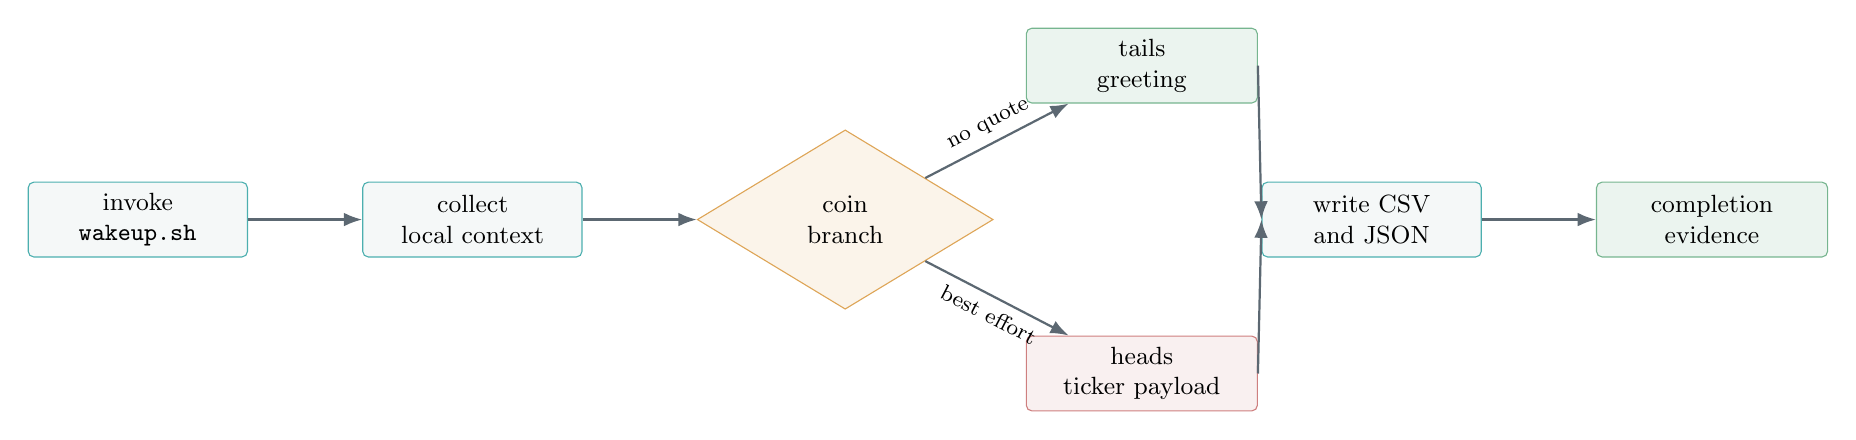
\begin{tikzpicture}[
  node distance=1.45cm,
  stage/.style={rectangle,rounded corners=2pt,draw=leafcyan!70,fill=leafpanel,
    text width=2.55cm,align=center,minimum height=0.95cm,font=\small},
  branch/.style={diamond,aspect=1.65,draw=leafamber!80,fill=leafamber!10,
    text width=2.15cm,align=center,font=\small},
  outnode/.style={rectangle,rounded corners=2pt,draw=leafgreen!70,fill=leafgreen!10,
    text width=2.7cm,align=center,minimum height=0.95cm,font=\small},
  warn/.style={rectangle,rounded corners=2pt,draw=leafred!70,fill=leafred!8,
    text width=2.7cm,align=center,minimum height=0.95cm,font=\small},
  arr/.style={-Latex,thick,draw=leafmuted}
]
\node[stage] (start) {invoke\\\texttt{wakeup.sh}};
\node[stage,right=of start] (ctx) {collect\\local context};
\node[branch,right=of ctx] (coin) {coin\\branch};
\node[outnode,above right=0.9cm and 1.35cm of coin] (tails) {tails\\greeting};
\node[warn,below right=0.9cm and 1.35cm of coin] (heads) {heads\\ticker payload};
\node[stage,right=3.4cm of coin] (logs) {write CSV\\and JSON};
\node[outnode,right=of logs] (gate) {completion\\evidence};

\draw[arr] (start) -- (ctx);
\draw[arr] (ctx) -- (coin);
\draw[arr] (coin) -- node[above,sloped,font=\footnotesize] {no quote} (tails);
\draw[arr] (coin) -- node[below,sloped,font=\footnotesize] {best effort} (heads);
\draw[arr] (tails.east) -- (logs.west);
\draw[arr] (heads.east) -- (logs.west);
\draw[arr] (logs) -- (gate);
\end{tikzpicture}
\end{center}

\subsection{Sparse Storage Pattern}

\tighttable
\begin{tabularx}{\linewidth}{@{}p{0.22\linewidth}p{0.24\linewidth}X@{}}
\toprule
Layer & Storage & Why it exists \\
\midrule
Compact event log & \texttt{wakeup\_log.csv} &
One row per branch execution. It is suitable for counts, rates, and quick result review. \\
Structured result & \texttt{wakeup\_result.json} &
Full object with branch, context, quote state, warning, message, and optional payload. \\
Latest pointer & \texttt{runs/latest/} &
Human-friendly access to the newest result without searching timestamps. \\
Completion map & \texttt{completion\_map.json} &
Proof that required files, logs, tests, and exports are present. \\
\bottomrule
\end{tabularx}
\normalsize

% ===========================================================================
\section{Results}

\subsection{Run Corpus Summary}

The sparse CSV contains ten branch events. Five are \texttt{heads}; five are
\texttt{tails}. All heads rows use ticker \texttt{NVDA}. All heads rows report
\texttt{module\_unavailable} because \texttt{yfinance} was not installed in the
run environment. This is a degraded data-collection state, not a node failure.

\begin{center}
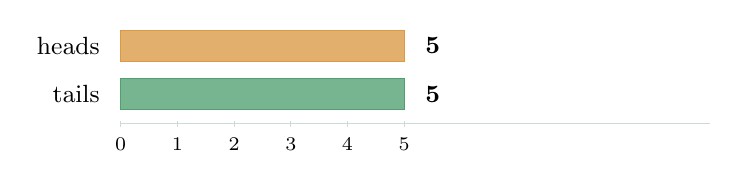
\begin{tikzpicture}[x=0.72cm,y=0.72cm]
  \draw[leafline] (0,0) -- (10.4,0);
  \draw[fill=leafamber!70,draw=leafamber!90] (0,1.1) rectangle (5,1.65);
  \draw[fill=leafgreen!70,draw=leafgreen!90] (0,0.25) rectangle (5,0.8);
  \node[anchor=east,font=\small] at (-0.2,1.38) {heads};
  \node[anchor=east,font=\small] at (-0.2,0.52) {tails};
  \node[anchor=west,font=\small\bfseries] at (5.2,1.38) {5};
  \node[anchor=west,font=\small\bfseries] at (5.2,0.52) {5};
  \foreach \x in {0,1,2,3,4,5} {
    \draw[leafline] (\x,0.05) -- (\x,-0.05);
    \node[font=\scriptsize,anchor=north] at (\x,-0.08) {\x};
  }
\end{tikzpicture}
\end{center}

\subsection{Sparse Log Rows}

\tighttable
\begin{tabularx}{\linewidth}{@{}p{0.28\linewidth}p{0.11\linewidth}p{0.13\linewidth}p{0.22\linewidth}X@{}}
\toprule
Local datetime & Branch & Ticker & Quote status & Warning \\
\midrule
2026-06-21T13:08:36-07:00 & tails & & & \\
2026-06-21T13:08:36-07:00 & heads & NVDA & module\_unavailable & yfinance not installed \\
2026-06-21T13:10:13-07:00 & tails & & & \\
2026-06-21T13:10:13-07:00 & heads & NVDA & module\_unavailable & yfinance not installed \\
2026-06-21T13:48:53-07:00 & tails & & & \\
2026-06-21T13:48:53-07:00 & heads & NVDA & module\_unavailable & yfinance not installed \\
2026-06-21T13:53:12-07:00 & tails & & & \\
2026-06-21T13:53:12-07:00 & heads & NVDA & module\_unavailable & yfinance not installed \\
2026-06-21T13:55:07-07:00 & tails & & & \\
2026-06-21T13:55:08-07:00 & heads & NVDA & module\_unavailable & yfinance not installed \\
\bottomrule
\end{tabularx}
\normalsize

\subsection{Snapshot Coverage}

The timestamped JSON folders contain six historical result snapshots. Four
timestamps in the CSV contain a tails row and a heads row in the same second.
The run directory name uses second-level time precision, so those paired tests
share the same folder key. The compact CSV preserves both events; the
timestamped folder preserves the last structured result for that second.

\begin{center}
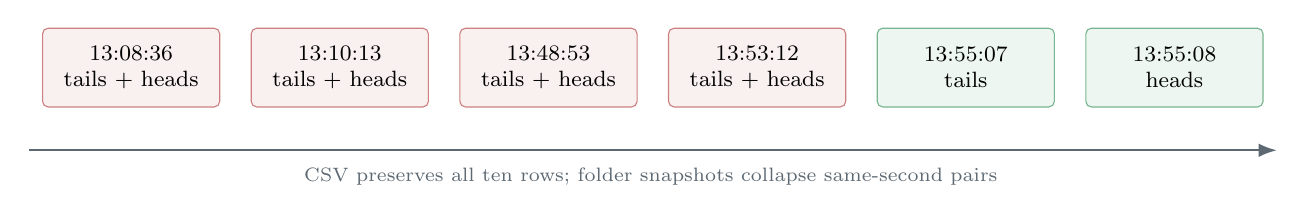
\begin{tikzpicture}[
  event/.style={rectangle,rounded corners=2pt,draw=leafline,fill=leafpanel,
    minimum width=2.25cm,minimum height=1.0cm,align=center,font=\footnotesize},
  collide/.style={rectangle,rounded corners=2pt,draw=leafred!70,fill=leafred!8,
    minimum width=2.25cm,minimum height=1.0cm,align=center,font=\footnotesize},
  ok/.style={rectangle,rounded corners=2pt,draw=leafgreen!70,fill=leafgreen!9,
    minimum width=2.25cm,minimum height=1.0cm,align=center,font=\footnotesize}
]
\node[collide] at (0,0) {13:08:36\\tails + heads};
\node[collide] at (2.65,0) {13:10:13\\tails + heads};
\node[collide] at (5.30,0) {13:48:53\\tails + heads};
\node[collide] at (7.95,0) {13:53:12\\tails + heads};
\node[ok] at (10.60,0) {13:55:07\\tails};
\node[ok] at (13.25,0) {13:55:08\\heads};
\draw[-Latex,thick,leafmuted] (-1.3,-1.05) -- (14.55,-1.05);
\node[anchor=north,font=\scriptsize\color{leafmuted}] at (6.6,-1.15) {CSV preserves all ten rows; folder snapshots collapse same-second pairs};
\end{tikzpicture}
\end{center}

\subsection{Quality And Degradation Matrix}

\tighttable
\begin{tabularx}{\linewidth}{@{}p{0.25\linewidth}p{0.22\linewidth}p{0.17\linewidth}X@{}}
\toprule
Result area & Observed state & Severity & Interpretation \\
\midrule
Branch coverage & 5 heads, 5 tails & pass &
Both deterministic branch paths were exercised evenly. \\
Structured result shape & latest JSON valid by schema intent & pass &
The result object carries branch, context, quote, message, and payload fields. \\
Optional quote module & yfinance missing on all heads rows & degraded &
The node continued and recorded \texttt{module\_unavailable}; this is expected behavior for optional data. \\
Run folder identity & same-second paired tests collapse to one folder key & action needed &
The sparse CSV is complete, but full JSON snapshots need a stronger run id. \\
Completion map & status verified & pass &
Required files, tests, logs, and export inclusion were recorded. \\
\bottomrule
\end{tabularx}
\normalsize

% ===========================================================================
\section{Methodology Findings}

\subsection{What The Sparse Design Proved}

\begin{itemize}
\item A compact CSV is excellent for branch counts, degradation rates, and
quick regression checks.
\item A full JSON result is the right shape for audit and replay, because it
keeps context, payload, and warning state together.
\item Degraded optional collection should be modeled as data, not as a crash.
\item The newest result pointer is useful for humans but should not be treated
as historical evidence.
\end{itemize}

\subsection{What The Runs Exposed}

The trial data exposed one important design issue: second-level timestamp
folders are not unique enough for rapid paired tests. The current naming
pattern is readable, but it is not collision-proof when two runs complete in
the same second.

Recommended next run identity:

\begin{lstlisting}[language={}]
runs/YYYY-MM-DD_HH-MM-SS-ms_WO-004-C_BRANCH_SEQ/
\end{lstlisting}

or:

\begin{lstlisting}[language={}]
runs/run_YYYYMMDDTHHMMSS_mmmZ_<short-random-or-counter>/
\end{lstlisting}

The CSV can remain sparse. The JSON directory should become collision-resistant.

% ===========================================================================
\section{Next Improvements}

\subsection{Visual And Data Improvements}

\tighttable
\begin{tabularx}{\linewidth}{@{}p{0.25\linewidth}p{0.20\linewidth}X@{}}
\toprule
Improvement & Target layer & Benefit \\
\midrule
Millisecond or monotonic run IDs & log writer &
Preserves every full JSON snapshot during fast paired branch tests. \\
Add \texttt{run\_id} to CSV and JSON & state contract &
Allows exact joins between sparse rows and structured result folders. \\
Add branch source field & methodology &
Separates random branch runs from forced branch coverage runs. \\
Record optional module state once & result context &
Makes \texttt{module\_unavailable} easier to distinguish from quote lookup failure. \\
Add a small generated summary file & reporting &
Lets future TeX/PDF reports rebuild tables from one stable artifact. \\
\bottomrule
\end{tabularx}
\normalsize

\subsection{Suggested Summary Object}

\begin{lstlisting}[language=json]
{
  "leafos_object": "sparse_game_run_summary",
  "version": "0.4.0-C",
  "source": "examples/WO-004-C/runs/wakeup_log.csv",
  "csv_rows": 10,
  "json_snapshots": 6,
  "branches": {"heads": 5, "tails": 5},
  "quote_status": {"module_unavailable": 5},
  "collision_note": "same-second paired tests share timestamp folder keys",
  "recommendation": "add run_id with milliseconds plus monotonic suffix"
}
\end{lstlisting}

% ===========================================================================
\section{Conclusion}

The sparse run method is worth keeping. It gives LeafOS a small, legible audit
trail while preserving enough structured data to reconstruct behavior. The
result set also made the next fix obvious: full JSON snapshots need a stronger
identity than second-level timestamps.

The best next version of this methodology is:

\begin{lstlisting}[language={}]
one compact row per event
one collision-resistant JSON folder per event
one latest pointer for humans
one generated summary for reports
one completion gate tying all of it together
\end{lstlisting}

That keeps the run system sparse, but no longer fragile under quick repeated
game trials.

\end{document}
